%%%%%%%%%%%%%%%%%%%%%%%%%%%%%%%%%%%%%%%%%%%%%%%%%%%%%%%%%%%%%%%%%%%%%%%%%%
% Cross-section of the power-loop copper over its return plane (Exercise 03, Task 1)
%%%%%%%%%%%%%%%%%%%%%%%%%%%%%%%%%%%%%%%%%%%%%%%%%%%%%%%%%%%%%%%%%%%%%%%%%%

\begin{figure}[htb]
	\begin{center}
		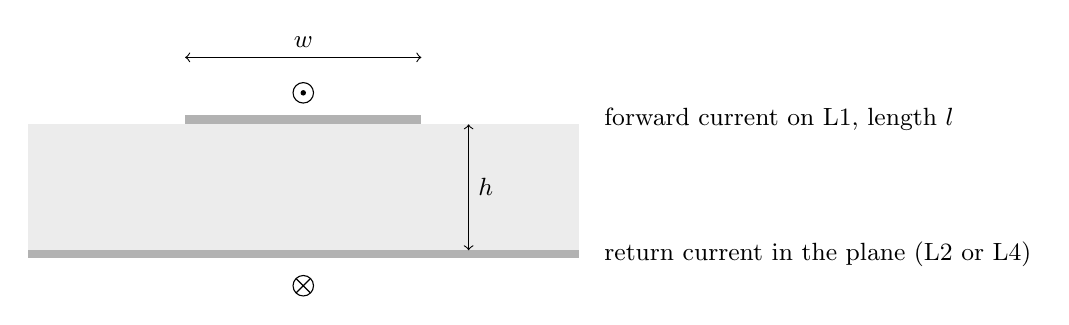
\begin{tikzpicture}[font=\small]
			% laminate, return plane and forward copper (not to scale)
			\fill[gray!15] (0,0) rectangle (7,1.6);
			\fill[gray!60] (0,-0.1) rectangle (7,0);
			\fill[gray!60] (2.0,1.6) rectangle (5.0,1.72);
			% current directions
			\draw (3.5,2.0) circle (0.13); \fill (3.5,2.0) circle (0.035);
			\draw (3.5,-0.45) circle (0.13);
			\draw (3.5,-0.45) ++(-0.09,-0.09) -- ++(0.18,0.18) ++(0,-0.18) -- ++(-0.18,0.18);
			% dimensions
			\draw[<->] (2.0,2.45) -- (5.0,2.45) node[midway, above] {$w$};
			\draw[<->] (5.6,0) -- (5.6,1.6) node[midway, right] {$h$};
			% labels
			\node[anchor=west] at (7.2,1.66) {forward current on L1, length $l$};
			\node[anchor=west] at (7.2,-0.05) {return current in the plane (L2 or L4)};
		\end{tikzpicture}
	\end{center}
	\caption{Cross-section of the power loop: forward copper of width $w$ over a solid return plane at the distance $h$ (not to scale).}
	\label{fig:ex03_loop}
\end{figure}
